\chapter{Dátové štruktúry: zásobník}
\label{sect:stack}
\def\stringcolor{solarized@blue}

Pokračujme v úlohe o klaunoch. Verzia \vb{klauni2} má kvadratickú zložitosť. 
Dá sa to ešte zlepšiť? Stále sa ešte robí dosť zbytočnej roboty: ak je medzi klaunom
\vb{i} a \vb{j} veľa malých klaunov, budeme ich testovať znova pri \vb{i+1}, \vb{i+2}
atď, aj keď je jasné, že už nikoho netrafia. Chceli by sme si preto pamätať
iba takých klaunov, ktorí ešte majú šancu niekoho trafiť. Na to ale potrebujeme
pomocné premenné, kde si ich uložíme, lebo vo vstupnom poli môžu byť na rôznych miestach.

\indexItem{Alg}{dátová štruktúra}
{\em Dátová štruktúra} je spôsob rozmýšľania o programe, ktorý pomáha rozdeliť program
na menšie nezávislé časti. Podobnú úlohu majú funkcie: v prvej verzii sme mali
funkciu \vb{trafi(j,i)}, ktorá testovala, či klaun \vb{j} trafí \vb{i}. V hlavnom
programe sme ju mohli používať a nestarať sa o to, ako je naprogramovaná vnútri, stačila
nám jej {\em špecifikácia}, t.j. charakteristika toho, čo robí. S dátovými 
štruktúrami je to podobné.
Povieme si, aké operácie potrebujeme s premennými vedieť robiť a zvlášť rozmýšľame o tom,
ako naprogramovať tie operácie a zvlášť o tom, ako s ich pomocou vyriešiť našu úlohu. 

 V našom prípade
použijeme dátovú štruktúru {\em zásobník} (stack).\indexItem{Alg}{zásobík} 
Zásobník je kopa vecí poukladaných na sebe. Dá
sa položiť vec na vrch, zobrať vec z vrchu a pozrieť sa, či je zásobník prázdny.
Ak dopredu vieme, aký najväčší zásobník budeme potrebovať, ľahko ho vyrobíme v poli.
Budeme mať pole \prg!int stack[n]! a premennú \prg!int m!, ktorá hovorí, koľko prvkov
je momentálne v zásobníku. Keďže prvky číslujeme od nuly, \vb{stack[m-1]} je 
prvok na vrchu, zobrať prvok z vrchu znamená urobiť \vb{m-=1} a pridať \vb{x} na vrch
znamená
\vb{stack[m]=x; m++}. 


S pomocou zásobníka vieme vylepšiť našu klaunskú úlohu. Keď testujeme klauna \vb{i},
budeme mať v zásobníku uložených všetkých kandidátov: t.j. klaunov, ktorých torty 
ešte letia vzduchom (modré prvky v ľavom obrázku sú v zásobníku pri spracovaní
klauna \vb{i}). Pri spracovaní klauna \vb{i} nepôjdeme doľava v pôvodnom poli,
ale iba v zásobníku (o klaunoch mimo zásobníka vieme, že ich torty aj tak
\vb{i}-čka netrafia). Pre všetkých menších ako \vb{i}, ktorých stretneme, 
zarátame zásah do \vb{i} a zároveň ich zo zásobníka vyhodíme, lebo za \vb{i}-čkom
už nikoho netrafia. Na obrázku vpravo je situácia po prechode na ďalšieho klauna.


\begin{column}{0.45}
  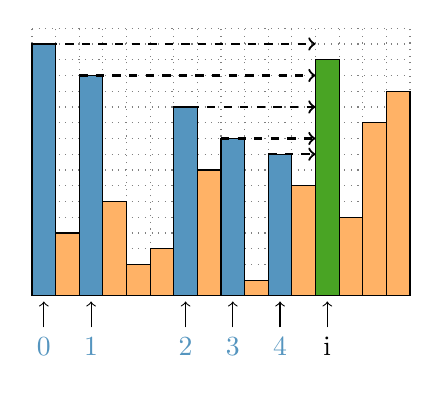
\begin{tikzpicture}[xscale=0.3,yscale=0.2]
  \draw[dotted,gray,thin] (1,0) grid (17,17);
  \def\bar(#1,#2)#3{
    \filldraw[draw=black,fill=#3](#1,0) rectangle (#1+1,#2);
  }
  \def\prf{orange!60!white}
  \def\rst{rgb:green,5;yellow,4;blue,2;black,3}
  \def\act{rgb:blue,5;green,3;white,4}
    \foreach \h [count=\i] in {16,4,14,6,2,3,12,8,10,1,9,7,15,5,11,13} {
    \bar(\i,\h){\prf}
  }
  \bar(13,15){\rst}
  \draw[->,shorten >= 2](13.5,-2) node[anchor=north]{\vb{i}} -- (13.5,0);

    \foreach \x/\h [count=\i]in {1/16, 3/14,7/12,9/10,11/9} {
    \bar(\x,\h){\act}
    \pgfmathtruncatemacro{\l}{\i-1}
    \draw[thick, dashed, ->](\x,\h)--(13,\h);  
    \draw[->,shorten >= 2](\x+.5,-2) node[anchor=north]{\vb{\textcolor{\act}{\l}} } 
    -- (\x+.5,0);

  }
  \end{tikzpicture}
\end{column}
\hfill
\begin{column}{0.45}
  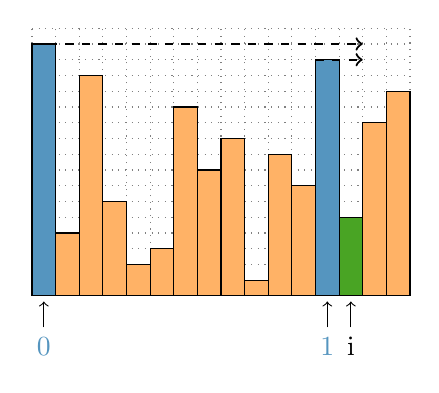
\begin{tikzpicture}[xscale=0.3,yscale=0.2]
  \draw[dotted,gray,thin] (1,0) grid (17,17);
  \def\bar(#1,#2)#3{
    \filldraw[draw=black,fill=#3](#1,0) rectangle (#1+1,#2);
  }
  \def\prf{orange!60!white}
  \def\rst{rgb:green,5;yellow,4;blue,2;black,3}
  \def\act{rgb:blue,5;green,3;white,4}
    \foreach \h [count=\i] in {16,4,14,6,2,3,12,8,10,1,9,7,15,5,11,13} {
    \bar(\i,\h){\prf}
  }
  \bar(14,5){\rst}
  \draw[->,shorten >= 2](14.5,-2) node[anchor=north]{\vb{i}} -- (14.5,0);
  
    \foreach \x/\h [count=\i]in {1/16,13/15} {
    \bar(\x,\h){\act}
    \pgfmathtruncatemacro{\l}{\i-1}
    \draw[thick, dashed, ->](\x,\h)--(15,\h);  
    \draw[->,shorten >= 2](\x+.5,-2) node[anchor=north]{\vb{\textcolor{\act}{\l}} } 
    -- (\x+.5,0);
  }
  \end{tikzpicture}
\end{column}


\vskip 1ex
\vbox{
\begin{lstlisting}[] 
int klauni3() {
  int i, max = 0;
  int s[n], m = 0;           // zásobník a jeho veľkosť
  for (i = 0; i < n; i++) {  // skúšame každého klauna
    int h = 0;               // koľko zásahov dostal
    while (m > 0 && s[m - 1] < a[i]) { // prechádzame zásobníkom až kým neprídeme
                                       // na začiatok alebo na vyššieho klauna
      h++;  // zarátame zásah
      m--;  // vyhodíme zo zásobníka
    }
    s[m] = a[i];  // pridáme i-čka do zásobníka
    m++;
    if (h > max) max = h;  // aktualizujeme zásahy
  }
  return max;
}
\end{lstlisting}
}


Akú má tento program zložitosť? Zdalo by sa, že sme si moc nepomohli, lebo stále
máme dva vnorené cykly, ale v skutočnosti každý prvok raz do zásobníka pridáme
a raz vyhodíme. Preto celková zložitosť bude lineárna. Ako vychádzajú skutočné časy?
Tentokrát som zobral som pre každé $n$ 500 náhodných 
vstupov a vyrátal priemerný čas (v mikrosekundách). 

\def\tmp#1{%
\begin{tikzpicture}
\begin{axis}[
    title={\vb{klauni#1}},  
  width=0.3*\textwidth, 
  height=7cm,
  xlabel={$n\cdot1000$},
  scaled x ticks=false,
  scaled y ticks=false,
  %domain=0:20000,
  xmin=0,
  %xmax=20000,
  /pgf/number format/.cd,
  1000 sep={},
  %legend cell align={left},
  %legend pos = south east
]
  \addplot+[no markers,orange!80!red] table 
  [y expr=\thisrow{v#1}, x expr=\thisrow{n}/1000 ]{data/klauni.dat};
\end{axis}
\end{tikzpicture}
\hfill
}

\tmp1
\tmp2
\tmp3


Vidno, že verzia \vb{klauni1} už na vstupoch dĺžky $8000$ (čo nie je nijak príliš veľa)
beží viac ako $1000$-krát pomalšie
oproti ostatným dvom. Medzi \vb{klauni2} a \vb{klauni3} taký veľký rozdiel nie je,
pretože na náhodných vstupoch sa aj vnútorný cyklus v \vb{klauni2} zastaví pomerne skoro.
Keď si ale pozrieme utriedený vstup, situácia sa zmení:

\def\tmp#1{%
\begin{tikzpicture}
\begin{axis}[
    title={\vb{klauni#1}},  
  width=0.3*\textwidth, 
  height=7cm,
  xlabel={$n\cdot1000$},
  scaled x ticks=false,
  scaled y ticks=false,
  %domain=0:20000,
  xmin=0,
  %xmax=20000,
  /pgf/number format/.cd,
  1000 sep={},
  %legend cell align={left},
  %legend pos = south east
]
  \addplot+[no markers,blue!20!cyan] table 
  [y expr=\thisrow{v#1}, x expr=\thisrow{n}/1000 ]{data/klauni2.dat};
\end{axis}
\end{tikzpicture}
\hfill
}

\hspace*{0.3\textwidth}\phantom{a}\hfill
\tmp2\tmp3


\begin{uloha}
  Na vstupe je pole $n$ čísel. Napíš program, ktorý pre každé 
  číslo vypíše pozíciu najbližšieho menšieho čísla vľavo, 
  alebo \vb{-1} ak také neexistuje.
  Napr. pre vstup \vb{5 2 3 4 3} treba vypísať \vb{-1 -1 1 2 1}.
\end{uloha}

\begin{uloha}
  Na vstupe je výraz zložený z rôznych druhov zátvoriek: \prg!'(',')','[',']','{','}'!.
  Vstup je ukončený znakom \vb{\$}.
  Napíš program, ktorý zistí, či sú zátvorky vyvážené a či každá otvorená zátvorka
  je uzavretá správnou zatváracou zátvorkou. Napr. výraz \vb{\textcolor{\stringcolor}{``({[](){}}())\$''}}
  aj \vb{\textcolor{\stringcolor}{``()\$''}}
  je správny, ale výraz \prg!"({])$"! ani \prg!")($"! nie je.
\end{uloha}

\begin{uloha}
  Napíš program, ktorý prečíta prirodzené číslo a vypíše jeho zápis v dvojkovej
  sústave.
\end{uloha}

\begin{uloha}
Naprogramuj úlohu \ref{uloha:vyrazy} bez rekurzie s použitím zásobníka.
\end{uloha}

\begin{uloha}
  \label{uloha:zatvorky}
Na vstupe je v prvom riadku číslo $n$ a v druhom riadku reťazec $n$ znakov 
zložený z malých písmen a zátvoriek. Zátvorky sú správne uzátvorkované.
Napíš program, ktorý vyrobí pole \vb{p} v ktorom pre každú pozíciu vstupu,
na ktorej je písmeno, bude \vb{-1} a pre pozície, kde je zátvorka, bude
pozícia zodpovedajúcej zátvorky. Napr. pre $n=25$ a reťazec 
  \vb{(o(atk)((nece)e(sarp)i)p)} má v poli \vb{p} byť
  \hbox{\vb{24 -1 6 -1 -1 -1 2 22 13 -1 -1 -1 -1 8 -1 20 -1 -1 -1 -1 15 -1 7 -1 0}}
\end{uloha}

\begin{uloha}
  Vstup je rovnaký ako v predchádzajúcej úlohe s tým, že prvý a posledný znak 
  sú zátvorky \prg!'(',')'!. Vstup predstavuje zašifrovaný text, ktorý treba 
  rozlúštiť takto: zober nejakú najvnútornejšiu dvojicu zátvoriek (t.j. otváraciu
  a zatváraciu zátvorku, medzi ktorými sú iba znaky), zátvorky zahoď a znaky medzi nimi
  otoč. Toto opakuj, kým sa neminú zátvorky. Napíš program, ktorý dešifruje text na vstupe.
  Ideálne by bolo, aby mal lineárnu zložitosť.
  Napr. pre vstup z predchádzajúcej úlohy je dešifrovaný text \vb{peceneprasiatko}.
\end{uloha}
